\section{Robottens bevægelse}
\label{RobottensBevaegelse}
%
Det vælges, at robotstyreren skal variere på robottens højde, afstand til testpersonen samt indgangsvinkelen, hvorved robotten henvender sig til en testperson. At netop de tre parametre er valgt skyldes, at det er muligt at ændre på dem ved brug af \textit{Double}. Formålet med at ændre på de tre fysiske parametre er at kunne undersøge, om de har indflydelse på nogen af de andre parametre.\blankline
%
Den laveste højde robotten kan have er 118 cm, målt fra gulvet til det øverste punkt på rammen hvori iPad'en sidder, hvor robotten maksimalt kan indstilles til en højde på 151 cm, målt fra gulv til top. De to højder vil derfor agere som de to ekstremer: \textit{Alt for lav} og \textit{Alt for høj}. På den bipolære skala, hvor robottens højde evalueres, er midtpunktet navngivet med: \textit{Fin}, som afspejler en højde svarende til omkring albuehøjde, jævnfør \fullref{ParametreDatabehandlingSkalaer}. Denne label er med til at kalibre skalaen, da der ikke findes en naturlig og logisk højde mellem de to ekstremer, hvorfor det vælges at én af højderne så vidt muligt skal afspejle, hvad testpersonerne forbinder med \textit{Fin}. For at have et kvalificeret estimat af albuehøjden tages der udgangspunkt i den gennemsnitligehøjde for danske mænd, som er 181.4 cm, og for danske kvinder, som er 167.2 cm, \parencite{WEB:DanskersHoejde}. Omregnes de to højder til en gennemsnitshøjde for danskere er højden 174.3 cm. Albuehøjden blev derfor målt ved, at en fra projektgruppen, som er ca. 174.3 cm høj, bukkede albueleddet i en vinkel på ca. 90$^\circ$ og interagerede med robotten i en højde, der føltes behageligt. Robottens højde blev målt til 129 cm når skærmen befandt sig i albuehøjde, hvilket svarer til midtpunktet på skalaen angivet med \textit{Fin}. Denne højde blev bekræftet af flere fra studiet, som blev spurgt om hvad de synes om robottens højde, hvortil de svarede: \textit{Fin}. 

For at få yderligere variation i robottens højde og for at præge testpersonerne til at bruge mere af skalaen, vælges det er inkludere to ekstra højder. Den ene højde er midt imellem minimum højden og albuehøjden, hvilket giver en højde på 123.5 cm målt fra gulv til top. Den anden højde er midt imellem albuehøjden og maks højden, hvilket giver en højde på 140 cm. Det tilstræbes, at indstille robotten i disse højder, dog kan der forekomme en lille variation i forhold til den eksakte højde. At der kan forekomme en lille variation i højden vurderes at være acceptabelt, da formålet med at ændre højden på robotten er at undersøge, hvilken indflydelse det kan have på andre parametre.\blankline           
%
I forhold til robottens afstand til testpersonerne vil tre afstande være gældende: Tæt på, tilpas og langt fra. Afstanden angives ikke i centimeter, da det ikke er muligt at sikre en specifik afstand, når robotten kører rundt i lufthavnen, i hvert fald ikke uden at forstyrre interaktionen mellem testperson og robot. Dog gør følgende retningslinjer sig gældende: Tæt på afspejler en afstand hvor robotten kommer så tæt på testpersonen, at testpersonen vil træde et skridt tilbage for at kunne interagere ordentlig på skærmen. En tilpas afstand afspejler en afstand, hvor testpersonen har mulighed for, at nå skærmen uden nødvendigvis at strække armen helt ud og uden at skulle træde et skridt tilbage. Afstanden langt fra afspejler at testpersonen med strakt arm ikke kan nå skærmen og derfor er nødsaget til at træde et skridt nærmere. Det forventes dog, at det ude i lufthavnen kan blive svært at overholde disse retningslinjer fuldt ud, da der vil forekomme situationer hvor de rejsende selv henvender sig til robotten og på den måde selv bestemmer en afstand. 

Den sidste af de tre parametre, der ændres på er: Robottens indgangsvinkel når den henvender sig til en potentiel testperson. Det vil blive forsøgt at få robotten til at henvende sig forfra, fra den rejsendes højre side og fra den rejsendes venstre side. Der sættes ikke krav til, at indgangsvinklen skal være præcis en samme hver gang den kommer fra enten højre eller venstre. Ligesom med afstanden forventes det dog, at det kan blive svært fuldstændigt at kunne kontrollere indgangsvinklen, da det dels afhænger af hvor mange rejsende der er i test området på det pågældende tidspunkt, hvor den rejsende befinder sig i forhold til robotten og dels afhænger af, om den rejsende selv henvender sig til robotten, da det i så fald vil være den rejsende, der dikterer indgangsvinklen.     

I \autoref{tab:Raekkefoelge} fremgår en plan for hvilken afstand robotten skal holde til testpersonen samt hvilken indgangsvinkel den skal henvende sig med når robotten er på sit laveste 118 cm. For at de fem højder alle præsenteres med de tre forskellige afstande og indgangsvinkler, resulterer det i 45 kombinationer. For de fire resterende højder vil rækkefølgen for afstand og indgangsvinkel være magen til den, der fremgår af \autoref{tab:Raekkefoelge}.    
%
\begin{table}[H]
	\centering 
	\begin{tabular}{c|c|c|c}
		Testperson  & Højde & Afstand & Indgangsvinkel \\\hline
		1   & 118 cm & Tæt på & Forfra  \\\hline
		2   & 118 cm & Tilpas & Forfra \\ \hline
		3   & 118 cm & Langt fra  & Forfra \\ \hline
		4   & 118 cm & Tæt på & Højre side \\ \hline
		5   & 118 cm & Tilpas & Højre side \\ \hline
		6   & 118 cm & Langt fra & Højre side \\ \hline
		7   & 118 cm & Tæt på & Venstre side \\ \hline
		8   & 118 cm & Tilpas & Venstre side \\ \hline
		9   & 118 cm & Langt fra  & Venstre side 
	\end{tabular} 
	\caption{Plan for hvilken afstand robotten skal have til testpersonen og hvilken indgangsvinkel den skal have ved henvendelse, når robotten er 118 cm høj. Tilsvarende er gældende for de fire resterende højder: 123.5 cm, 129 cm, 140 cm og 151 cm.}
	\label{tab:Raekkefoelge}       
\end{table}
\noindent
%
For at opnå de 45 kombinationer af højde, afstand og indgangsvinkel kræver det deltagelse fra minimum 45 testpersoner. Det tilstræbes, at have alle 45 testpersoner på én dag, men da der kun blev udført 18 interviews i feltundersøgelsen, jævnfør \fullref{ParametreFaktiskeTestpersoner}, er det ikke sikkert at det er muligt. Er det ikke muligt, at indsamle data fra minimum 45 testpersoner på én dag vil testen foretages over flere dage til det ønskede antal testpersoner er opnået.   

\section{Rollefordeling}
\label{TestAfSkalaRollefordeling}
%
For at udføre testen er det nødvendigt at definere nogle roller, hvortil specifikke opgaver tildeles. Der opstilles i alt tre forskellige roller. 
%
\subsubsection*{Robotstyrer}
%
Som ved feltundersøgelsen vælges det ligeledes at fjernstyre \textit{Double}-robotten, hvorfor det er nødvendigt at have en person til at styre robotten. Robotstyren har til opgave at køre robotten rundt i lufthavnen og få den til at henvende sig til de rejsende i området. Hvordan robotten skal bevæge sig i forhold til afstanden til testpersonen og indgangsvinklen for henvendelse fremgår af \autoref{tab:Raekkefoelge}.

\subsubsection*{Observatør af interaktion på skærmen}
%
Observatøren skal holde øje med, hvad de rejsende trykker på skærmen. Hvis der trykkes \textit{Nej} skal observatøren indikere til robotstyreren, at robotten skal køre væk. Dette indikeres ved, at observatøren vender tommelfingeren nedad. Hvis den rejsende, der interagerer med robotten, trykker \textit{Ja}, skal observatøren holde øje med, hvornår der står: \textit{Følg venligst efter mig} på skærmen. Dette indikeres ved, at observatøren vender tommelfingeren opad, hvorefter robotstyreren lader robotten køre mod shoppingområdet. 

\subsubsection*{Observatør af robotten}
%
Personen med denne rolle har til opgave at observere og notere, hvordan robotten bevæger sig i forhold til om det stemmer overens med robotstyrens plan, jævnfør \autoref{tab:Raekkefoelge}. De parametre, der er særlig vigtige at notere er:\blankline 
%
\begin{itemize}
	\item Højde
	\item Afstand
	\item Indgangsvinkel\blankline
\end{itemize}
\noindent
%
I tilfælde af, at robotten bevæger sig anderledes end hvad den plejer skal dette ligeledes noteres af observatøren. Vurderer observatøren, at der er andre hændelser, der er vigtige at have til senere brug, noteres disse. Formålet med denne observatør er at indsamle data, der kan være relevant for hvordan robotten agerede ved den enkelte testperson i henhold til testpersonens evaluering.

\subsubsection*{Testleder}
%
Testlederens opgave er at henvende sig til testpersonen, når robotten følger dem mod shoppingområdet, og spørger dem om de har tid til at svare på nogle spørgsmål. Spørgsmålene er skalaerne. Har testpersonen tid til at evaluere sin oplevelse på skalaerne følger testlederen dem hen til bordet, hvor de præsenteres for skalaerne på computeren. Testlederen har i den forbindelse til opgave at notere testpersonnummer i programmet, jævnfør \fullref{TestAfSkalaProgramSkala}, og efterfølgende eksekvere programmet, så testpersonen kan svare på skalaerne. Testlederen har desuden til opgave at observere og svare på spørgsmål vedrørende skalaerne, hvis testpersonen måtte have nogle. Dette vil testlederen sørger for at notere. 

Det er vigtigt at testlederen, i tilfælde hvor testpersonen har spørgsmål til skalaerne, ikke forklarer projektgruppens forståelse af spørgsmålet, men i stedet lader det være op til den enkelte testpersonen at danne sin egen forståelse af spørgsmålet. Det kan eksempelvis gøres ved, at testlederen siger: \textit{Det er ud fra din forståelse af det} eller \textit{Hvad synes du det betyder?}. Efter testpersonen har besvaret alle skalaer og udfyldt demografien, takker testlederen testpersonen for sin deltagelse og ønsker dem en god rejse.
\newpage
 
\section{Demografi}
\label{Demografi}
%
Testpersonerne vil blive bedt om at udfylde demografi, som indeholder køn, alder, højde, hvor ofte testpersonen rejser og hvor meget kendskab de har til teknologi. Demografien fremgår af \autoref{fig:Demografi}.
%
\begin{figure}[H]
\centering
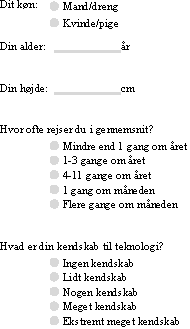
\includegraphics[width = 0.45\textwidth]{Figure/TestdesignEvaluering/Demografi} 
\caption{Demografi, som testpersonen skal udfylde efter skalaerne er besvaret.}
\label{fig:Demografi}
\end{figure}
\noindent
%
Kønnet kan enten angives som \textit{Mand/dreng} eller \textit{Kvinde/pige} årsagen til, at dreng og pige indgår i demografien er, at i feltundersøgelsen var en af testpersonerne kun 8 år, hvorfor det forventes at have børn som testpersoner igen. Derudover er det ikke sikkert, at et barn identificerer sig som mand eller kvinde, hvorfor dreng og pige er noteret. Alder noteres for at vide hvor stort et spænd testpersonerne dækker over, da det tidligere er fundet, at der kan være aldersforskelle i forhold til interaktionen med sociale robotter. Højden noteres i centimeter for, at have sammenholde det med robottens højde i forhold til evalueringen, da det kan have indflydelse på nogle af parametrene. 

I den foregående feltundersøgelse blev testpersonerne spurgt, hvor ofte de rejser. Det vælges at få testpersonerne til at notere, hvor ofte de rejser istedet for at spørger dem, da deres respons desværre var svær at fortolke og kategorisere. Nogen af testpersonerne svarede nemlig, at de rejser ofte, men det er uvist hvad ofte egentligt er.   

Som tidligere nævnt vil spørgsmålet omkring testpersonernes kendskab til teknologi/robotter blive stillet i forbindelse med demografien. I det henseende er det valgt at formulere spørgsmålet som: \textit{Hvad er din kendskab til teknologi} og istedet for en skala, besvares spørgsmålet på en \textit{Likert-scale}, hvor graden af kendskab fremgår i fem niveuaer. At teknologi vælges frem for robotter skyldes, at teknologi er mere dækkende for har testpersonerne kendskab til robotter, så har de også kendskab til teknologi, men har de kendskab til teknologi er det ikke ens betydende med, at de har kendskab til robotter.

\section{Testlokation og udstyr}
\label{TestAfSkalaLokationUdstyr}
%
De ændringer, der er til testlokation og udstyr i forhold til hvordan det er beskrevet i \fullref{ParametreTestlokationOgUdstyr}, henvender sig blandt andet til hvad der var muligt at gøre i lufthavnen, og er beskrevet i \fullref{ParametreTestdesign}. Udover de ændringer, vil der blive anvendt en computer hvorpå skalaerne præsenteres, computeren er en: \textit{Microsoft Surface Pro (5)}, hvis skærm er 12.3" med en opløsning på 2736 x 1824, dertil vil der være en trådløs mus til rådighed, som testpersonerne skal bruge til at markere det sted på skalaen, der er deres respons. I modsætning til feltundersøgelsen, hvor demografien indsamlet ved at stille testpersonerne spørgsmål, er der til denne test blevet udviklet et ark hvorpå testpersonerne selv kan notere informationerne. 

Derudover vil testlederen ikke optage hvad testpersonen siger, da der som udgangspunkt ikke blive stilt spørgsmål. Stilles der spørgsmål vil det blive noteret af testlederen på papir. 


